\documentclass[graphics]{beamer}

\usepackage{graphicx}
\usepackage{verbatim}
\usepackage{wrapfig}
\useoutertheme{shadow}
%\usecolortheme{orchid}
\usecolortheme{seahorse}


% math commands
\newcommand{\be}{\begin{eqnarray}}
\newcommand{\ee}{\end{eqnarray}}
\newcommand{\beq}{\begin{equation}}
\newcommand{\eeq}{\end{equation}}
\def\simless{\mathbin{\lower 3pt\hbox
      {$\rlap{\raise 5pt\hbox{$\char'074$}}\mathchar"7218$}}}
\def\simgreat{\mathbin{\lower 3pt\hbox
      {$\rlap{\raise 5pt\hbox{$\char'076$}}\mathchar"7218$}}} %> or of order

% variables

\def\toonscale{0.45}
\def\mboxy#1{\mbox{\small #1}}


\begin{comment}
\AtBeginSection[]{
  \frame{
    \frametitle{Outline}
    \tableofcontents[currentsection]
  }
}
\end{comment}

\title{Imaging the ISM through pulsars
}
%\subtitle{interim update}
\author[U. Pen]{Ue-Li Pen and collaborators
}
\date{May 15, 2024}


\begin{document}

%\section*{Introduction}
\section{Lenses}

\begin{comment}
  \subsection{Outline}

  \frame{
    \frametitle{Outline}
    \tableofcontents
  }
\end{comment}

\frame{\maketitle}




  \frame{
    \frametitle{Coherent sources: Pulsars, FRBs}
    \begin{itemize}
        \item Coherent, distant source of radiation, highest known
          brightness temperature
        \item Scintillate under multi-path propagation          
        \item sensitive to ns time delay propagating for gigaparsecs
    \end{itemize}
  }


  \frame{

    \frametitle{PSR B0834+06: Coherent VLBI}
\vspace{-0.25in}
\begin{center}
\hspace{-0.5in}
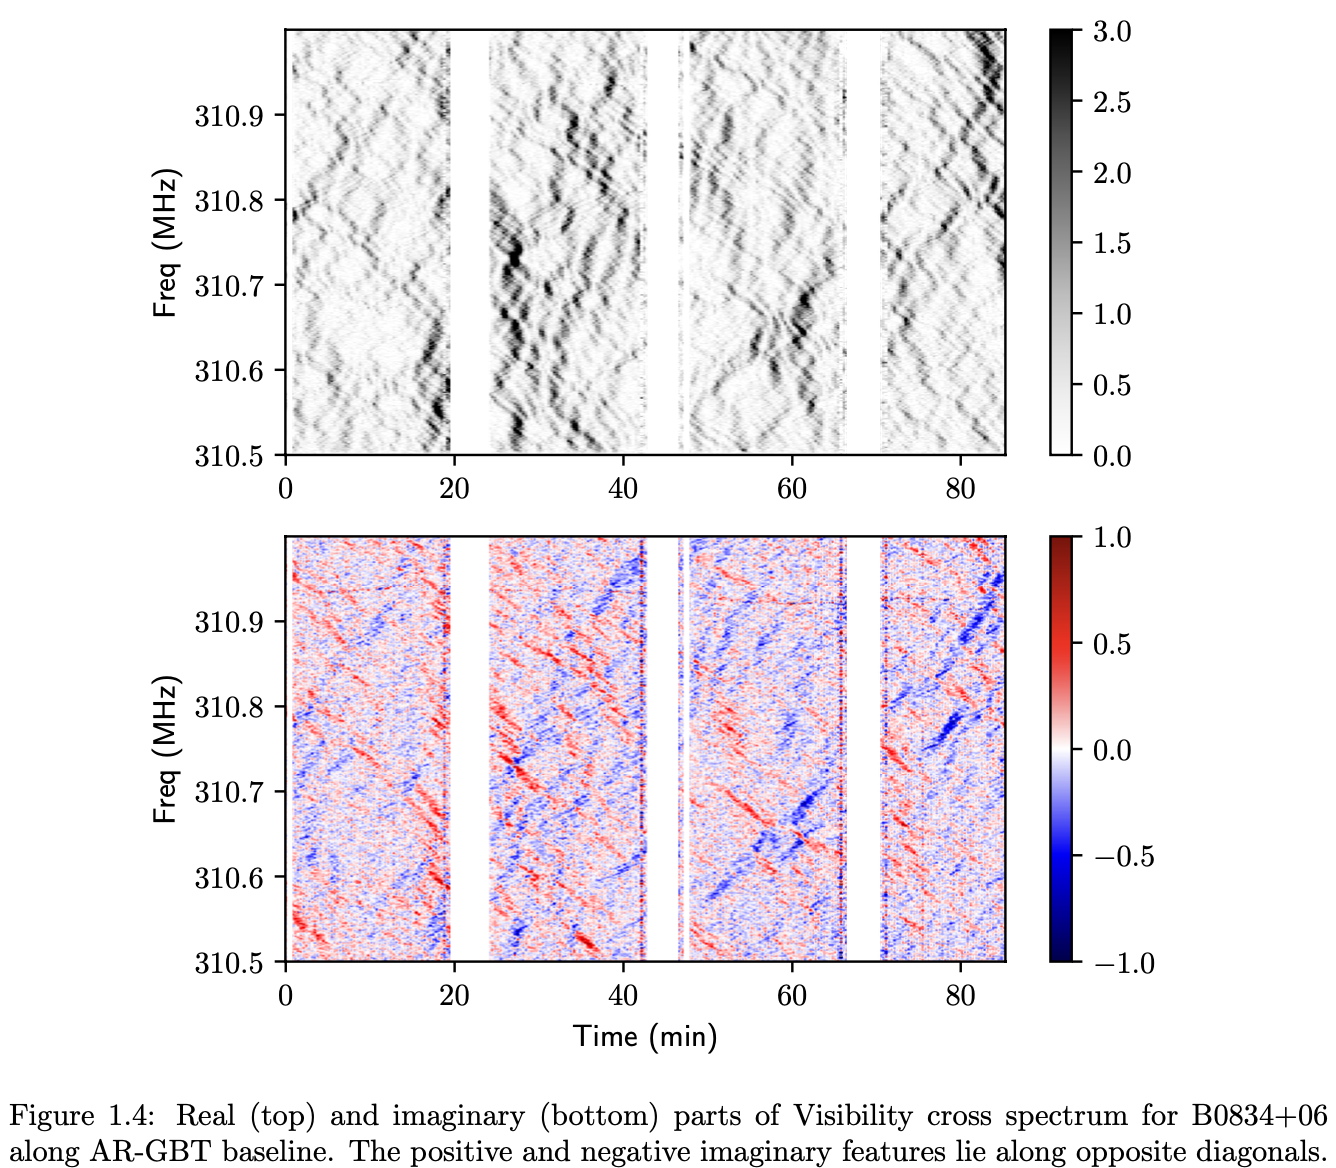
\includegraphics[width=3.5in]{Figures/rawvlbi.png}
\end{center}
  }

    \frametitle{PSR B0834+06: Brisken}
\vspace{-0.25in}
\begin{center}
\hspace{-0.5in}
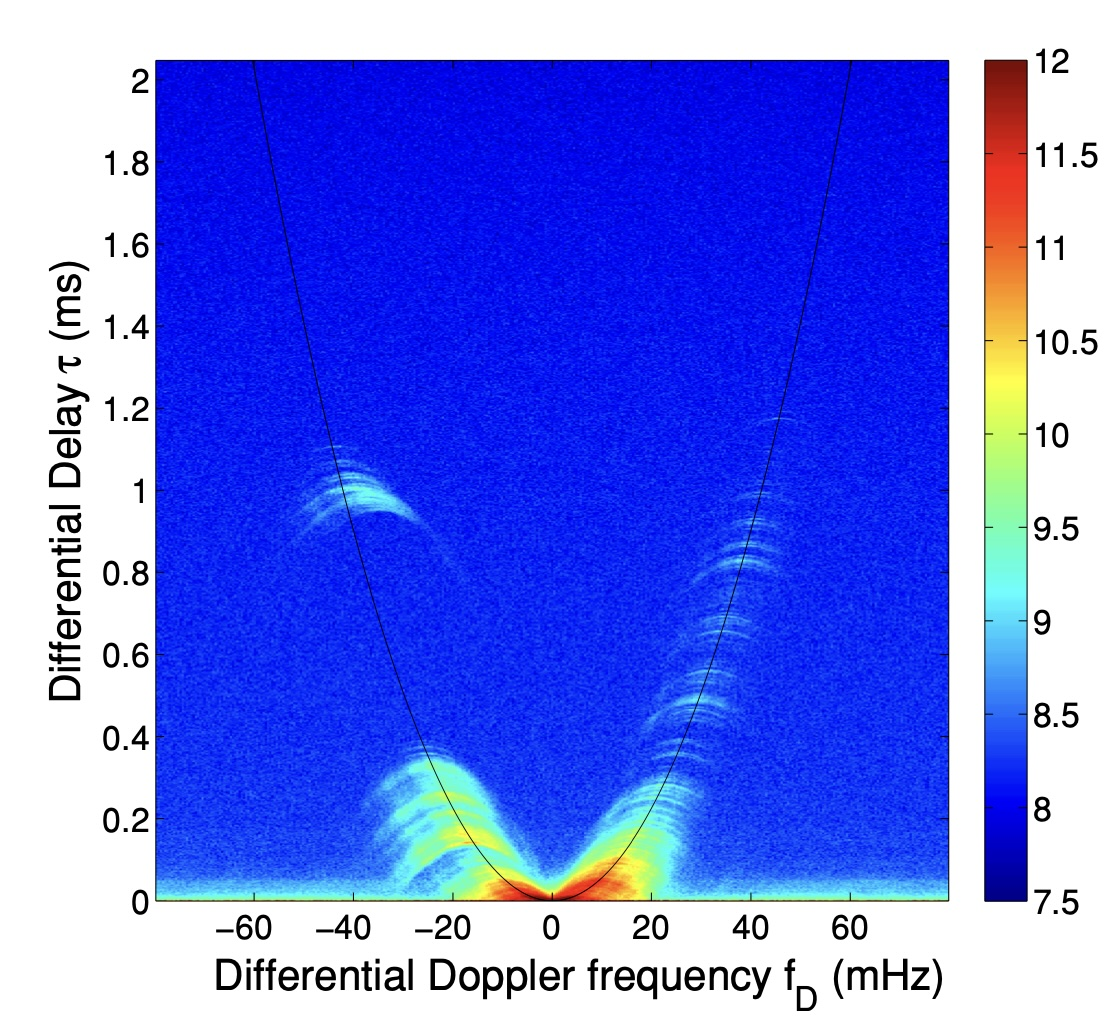
\includegraphics[width=3.5in]{Figures/briskenarc.jpg}
\end{center}
  }



  \frame{
%\vspace{-0.25in}
    \frametitle{Scintillometry VLBI}
\hspace{-0.25in}
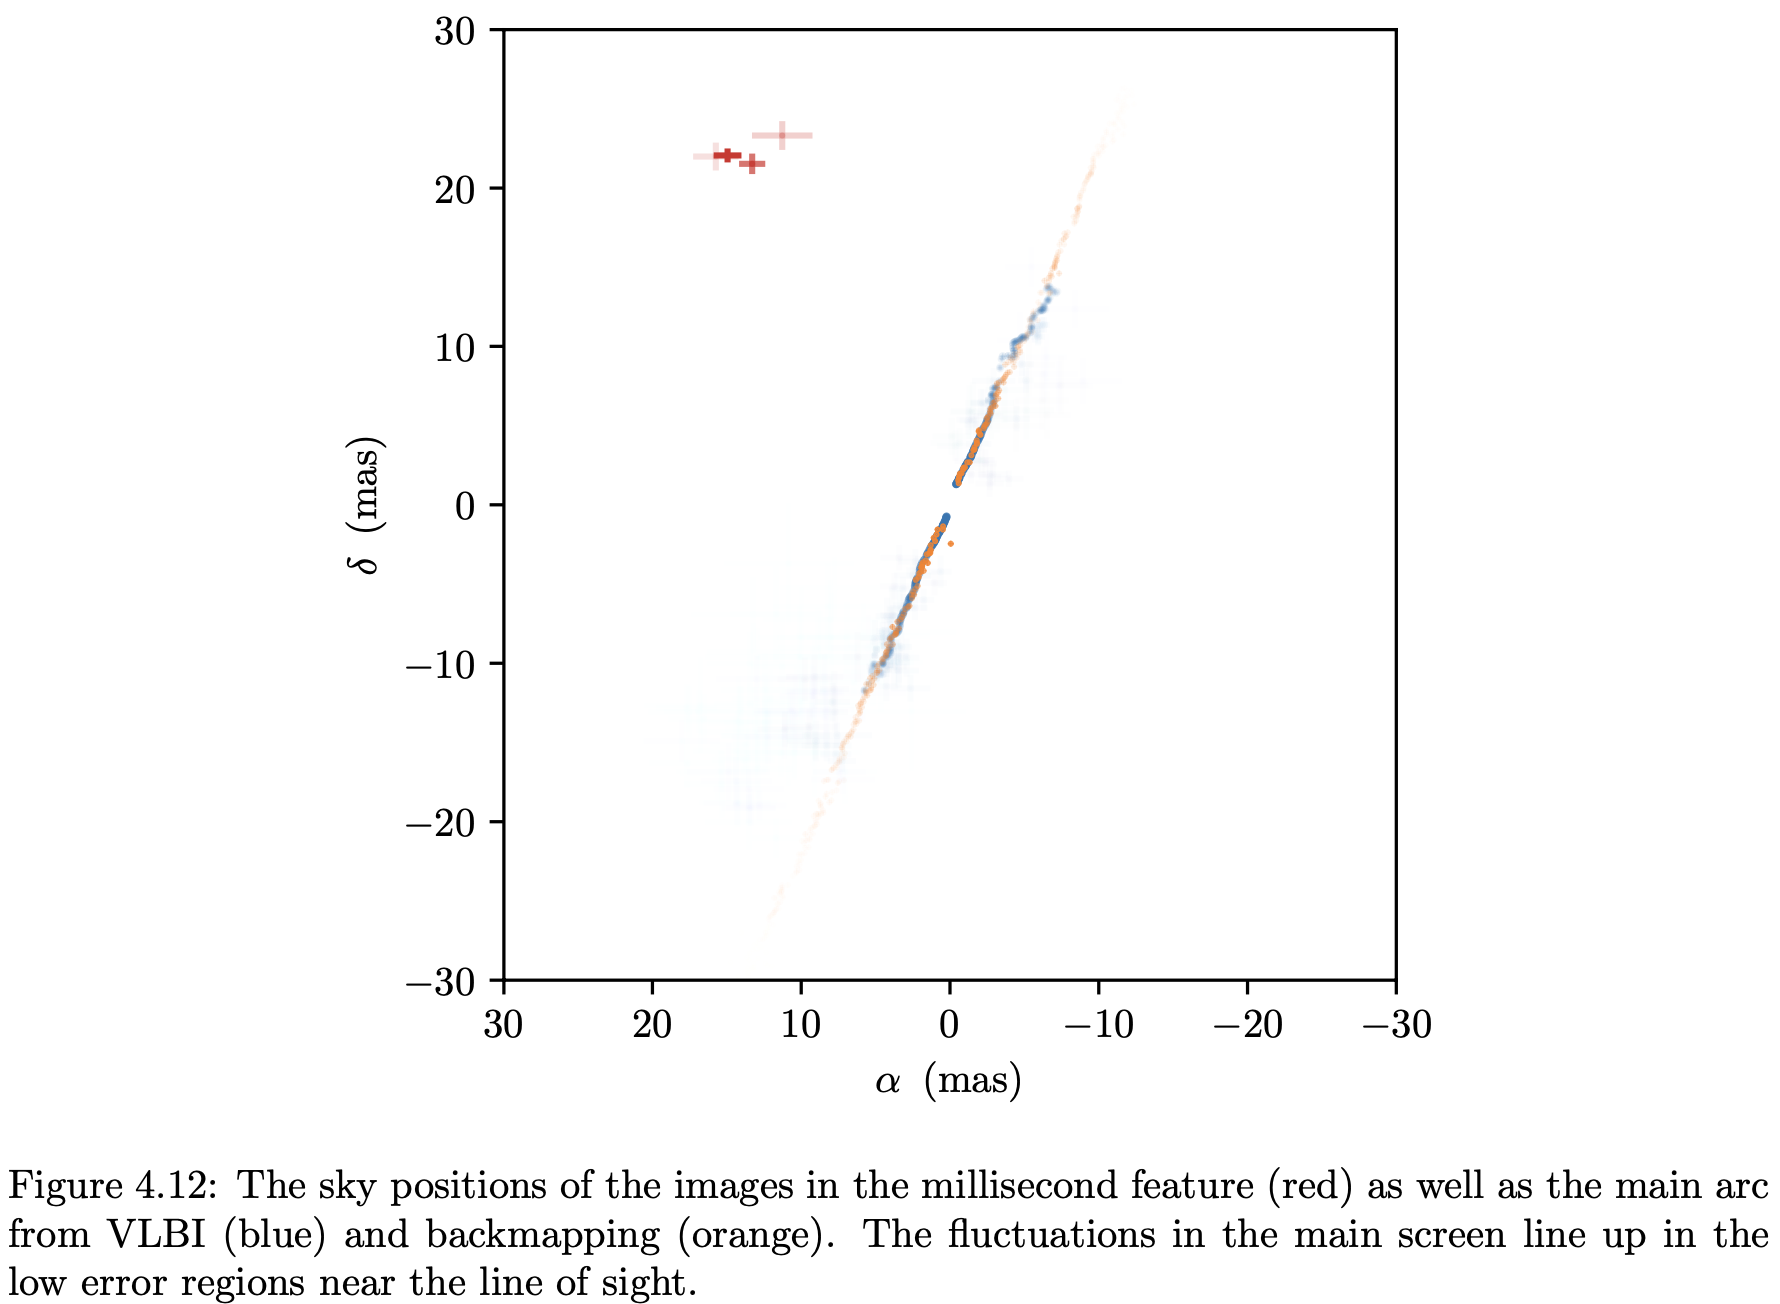
\includegraphics[width=3.5in]{Figures/VLBI0834.png}
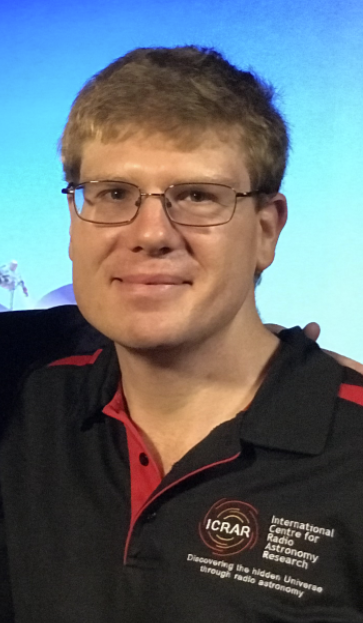
\includegraphics[width=1.05in]{Figures/jpm.png}

Baker++: highly linear lenses!
  }

    \frametitle{PSR B0834+06: Zhu}
\vspace{-0.25in}
\begin{center}
\hspace{-0.5in}
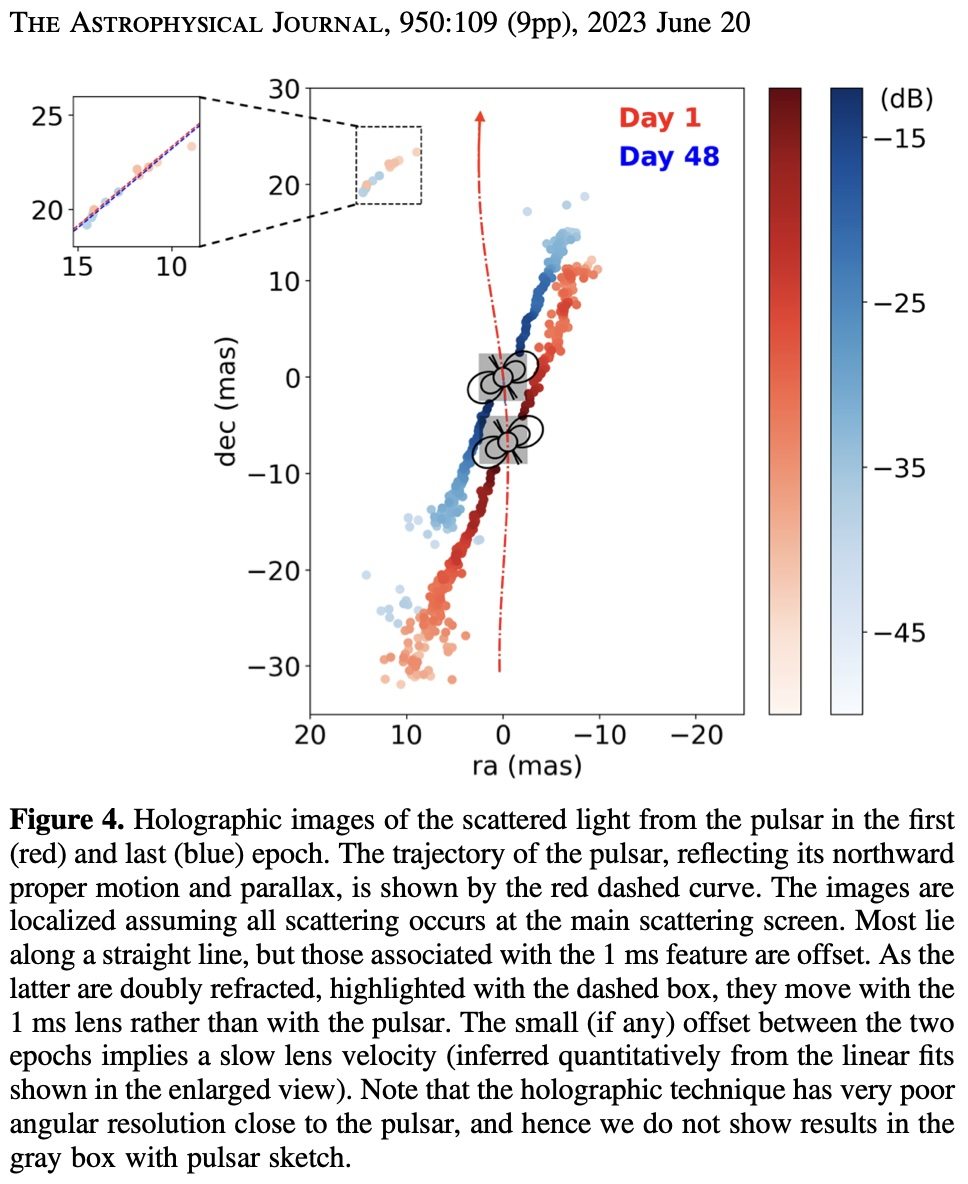
\includegraphics[width=3.5in]{Figures/zhuese.jpg}
\end{center}
  }


\frame{
    \frametitle{Toronto}
     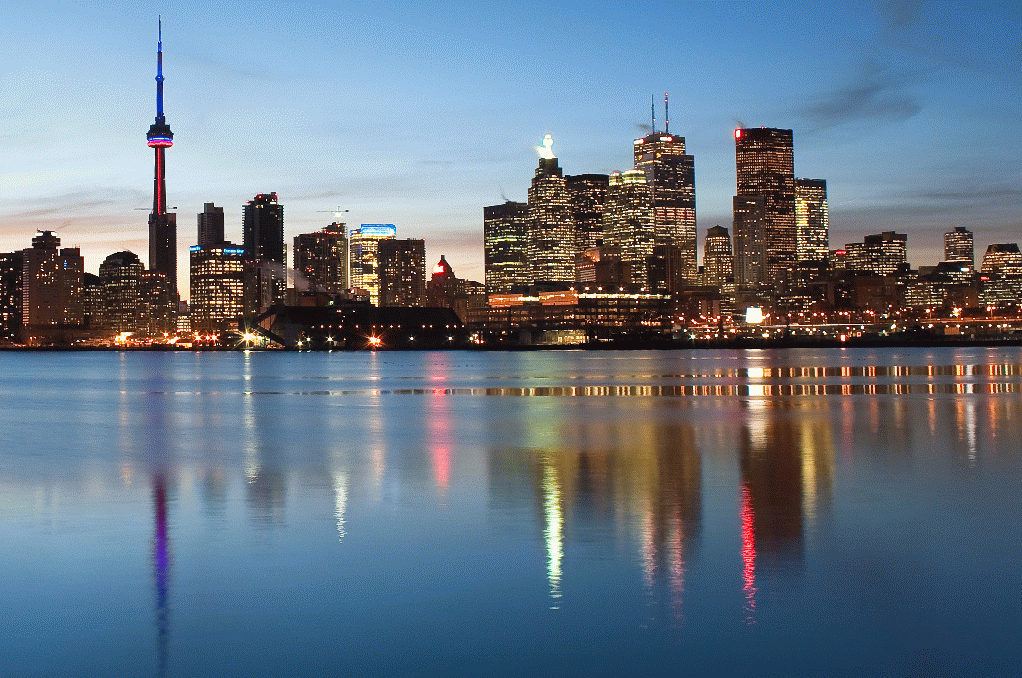
\includegraphics[width=\textwidth]{Figures/toronto-skyline.png}

\tiny Liu et al 2015, arvix:1507.00884
}


  \frame{
    \frametitle{Lensing}
    \begin{itemize}
      \item underdense $\longrightarrow$ convergent
      \item overdense $\longrightarrow$ divergent
      \item fold $\longrightarrow$ violate odd image theorem
      \item only one image per wave period, not 4
    \end{itemize}
\vspace{-0.75in}\hspace{3.5in}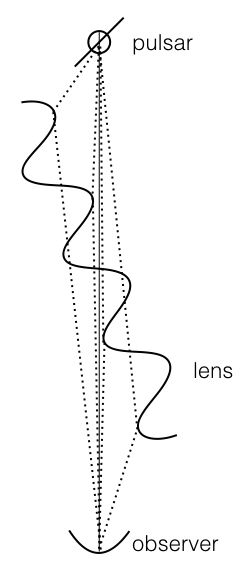
\includegraphics[width=0.25\textwidth]{Figures/convergent_geometry.jpeg}
  }

  \frame{
%\vspace{-0.5in}
    \frametitle{Ducted Alven waves}
    \begin{itemize}
     \item magnetic fields in equilibrium like to be straight
      \item domain boundaries where fields change discontinuously
      \item surface Alven waves propagate along these sheets
      \item blazing may cause asymmetric arcs
    \end{itemize}
  }


  \frame{
%\vspace{-0.5in}
    \frametitle{Goldreich-Shridar 2006}
    \begin{itemize}
     \item corrugated sheets
      \item scattering dominated by most inclined sheet
      \item explains why many lines of sight dominated by single lens system
    \end{itemize}
  }

  \frame{

    \frametitle{precision astrometry}
\vspace{-0.25in}
\begin{center}
\hspace{-0.5in}
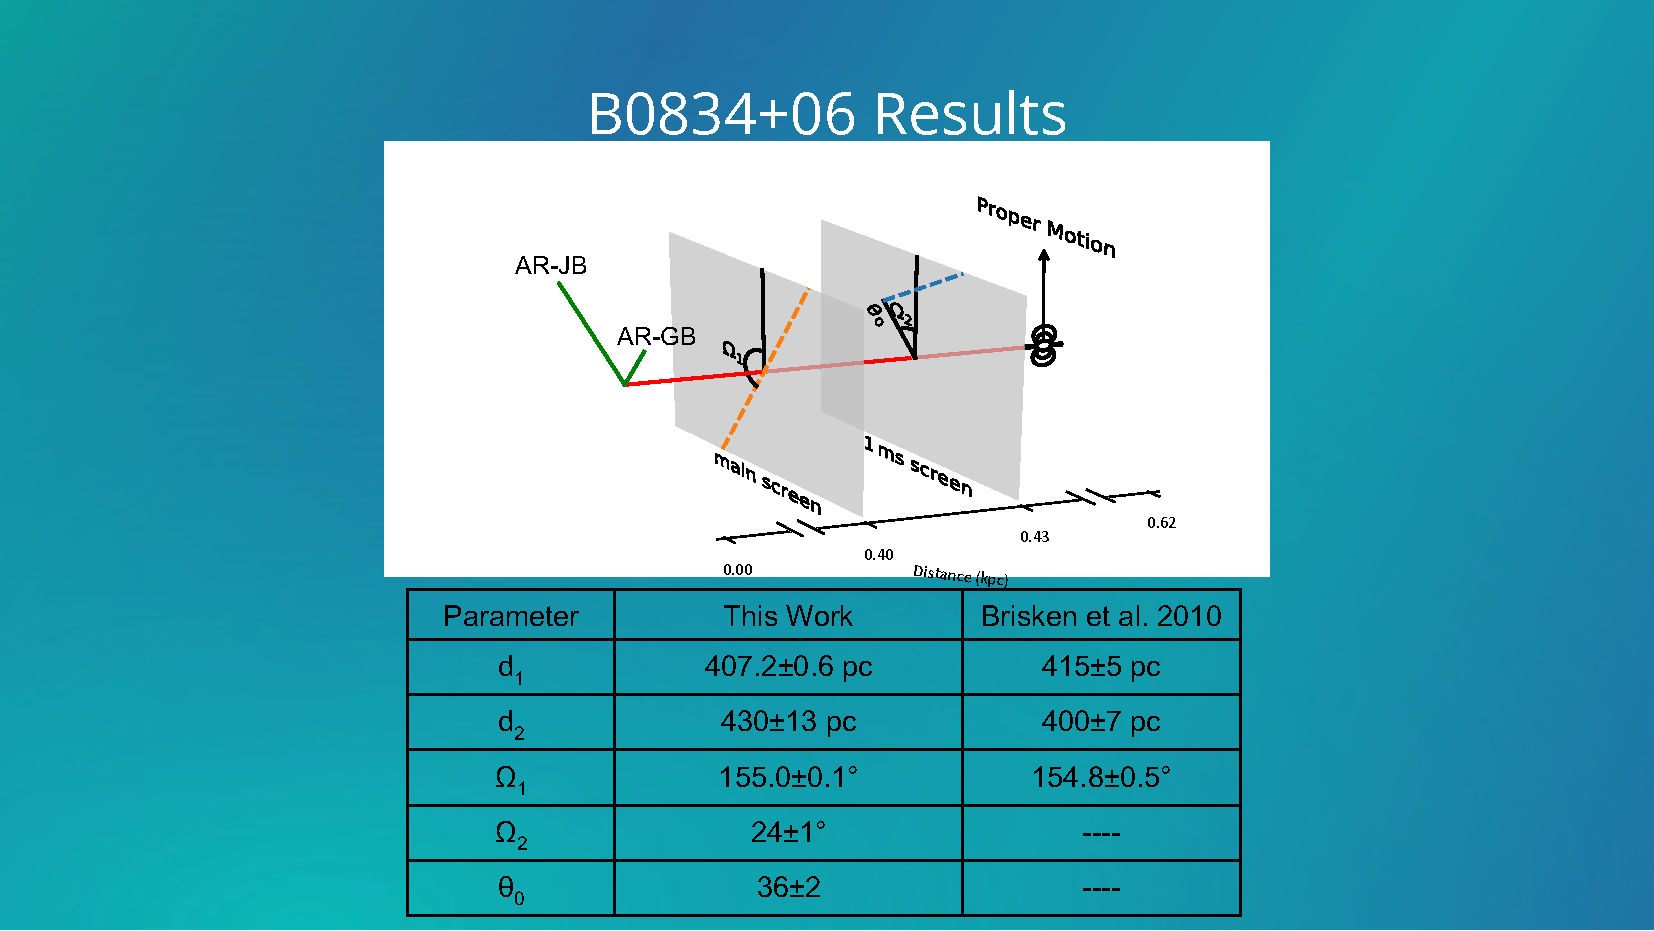
\includegraphics[width=5.5in]{Figures/VLBIdist.pdf}
\end{center}
  }


  \frame{

    \frametitle{more precision astrometry}
%\vspace{-0.25in}
\begin{center}
%\hspace{-0.5in}
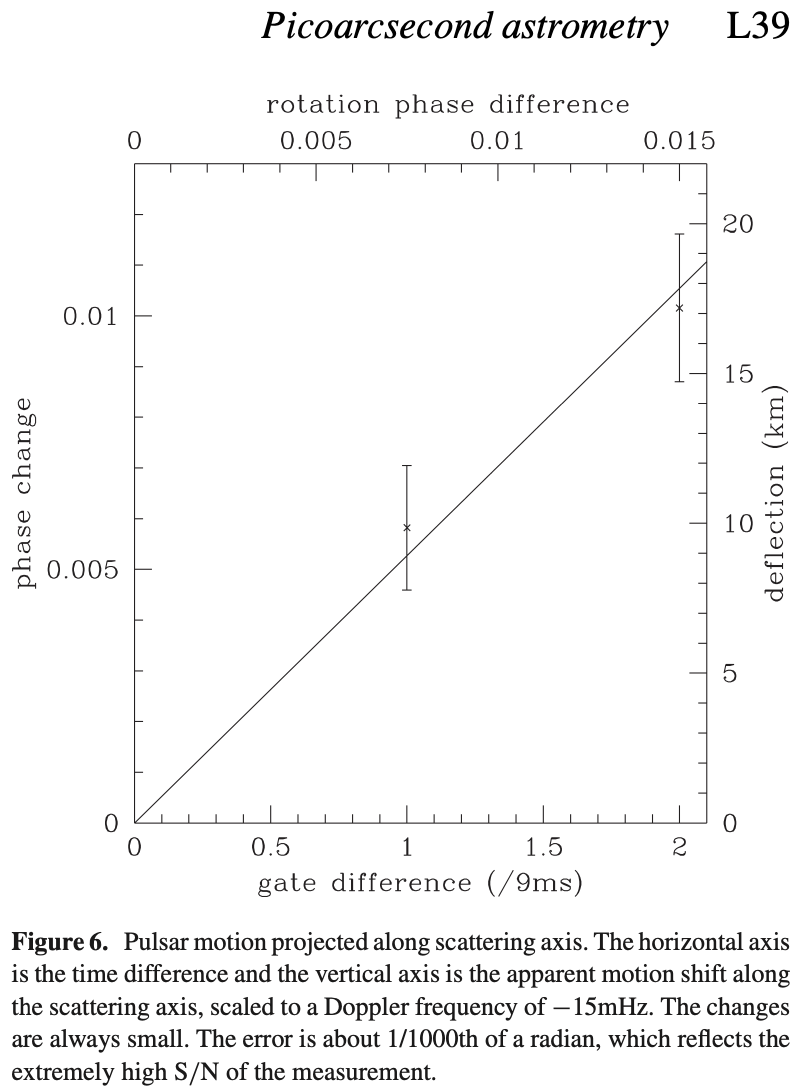
\includegraphics[width=2.05in]{Figures/pico.png}
UP+14
\end{center}
  }



  \frame{

    \frametitle{Catastrophes}
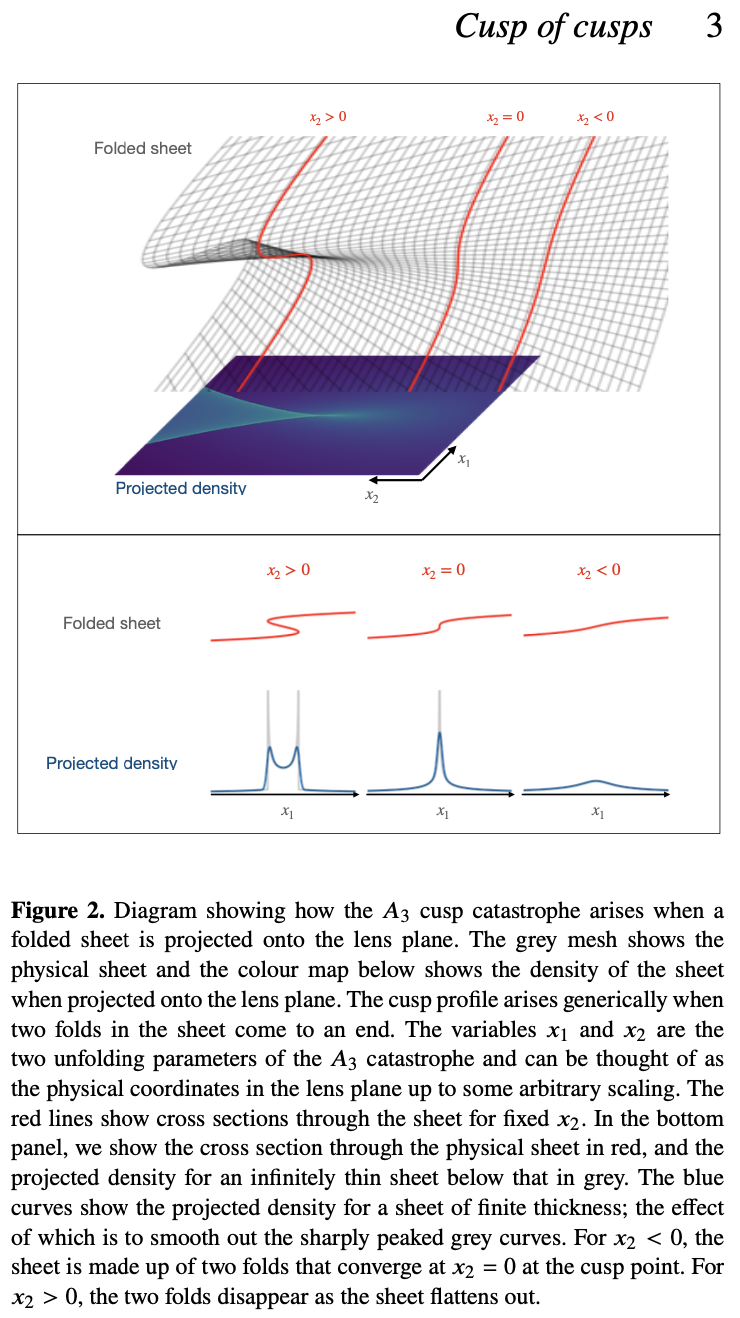
\includegraphics[width=2.85in]{Figures/cusp.png}
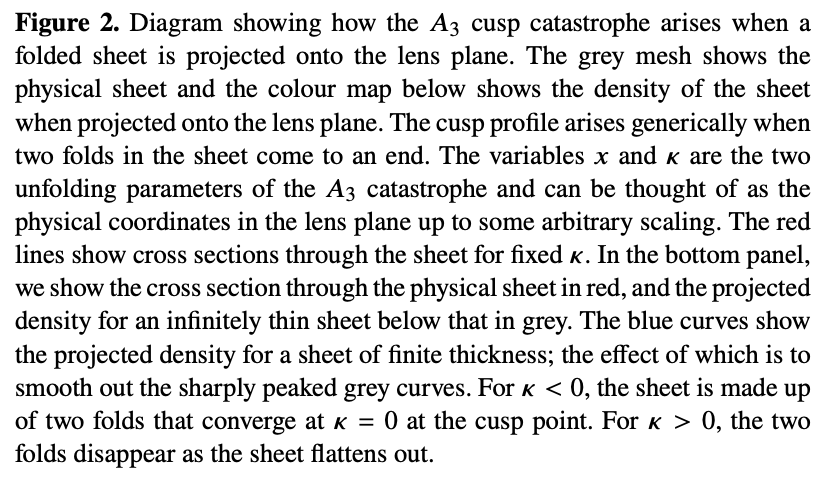
\includegraphics[width=0.5in]{Figures/cuspcaption.png}
Jow+2301.08344
  }

  \frame{
    \frametitle{Extreme Scattering Events}
%\hspace{-0.5in}
\begin{center}
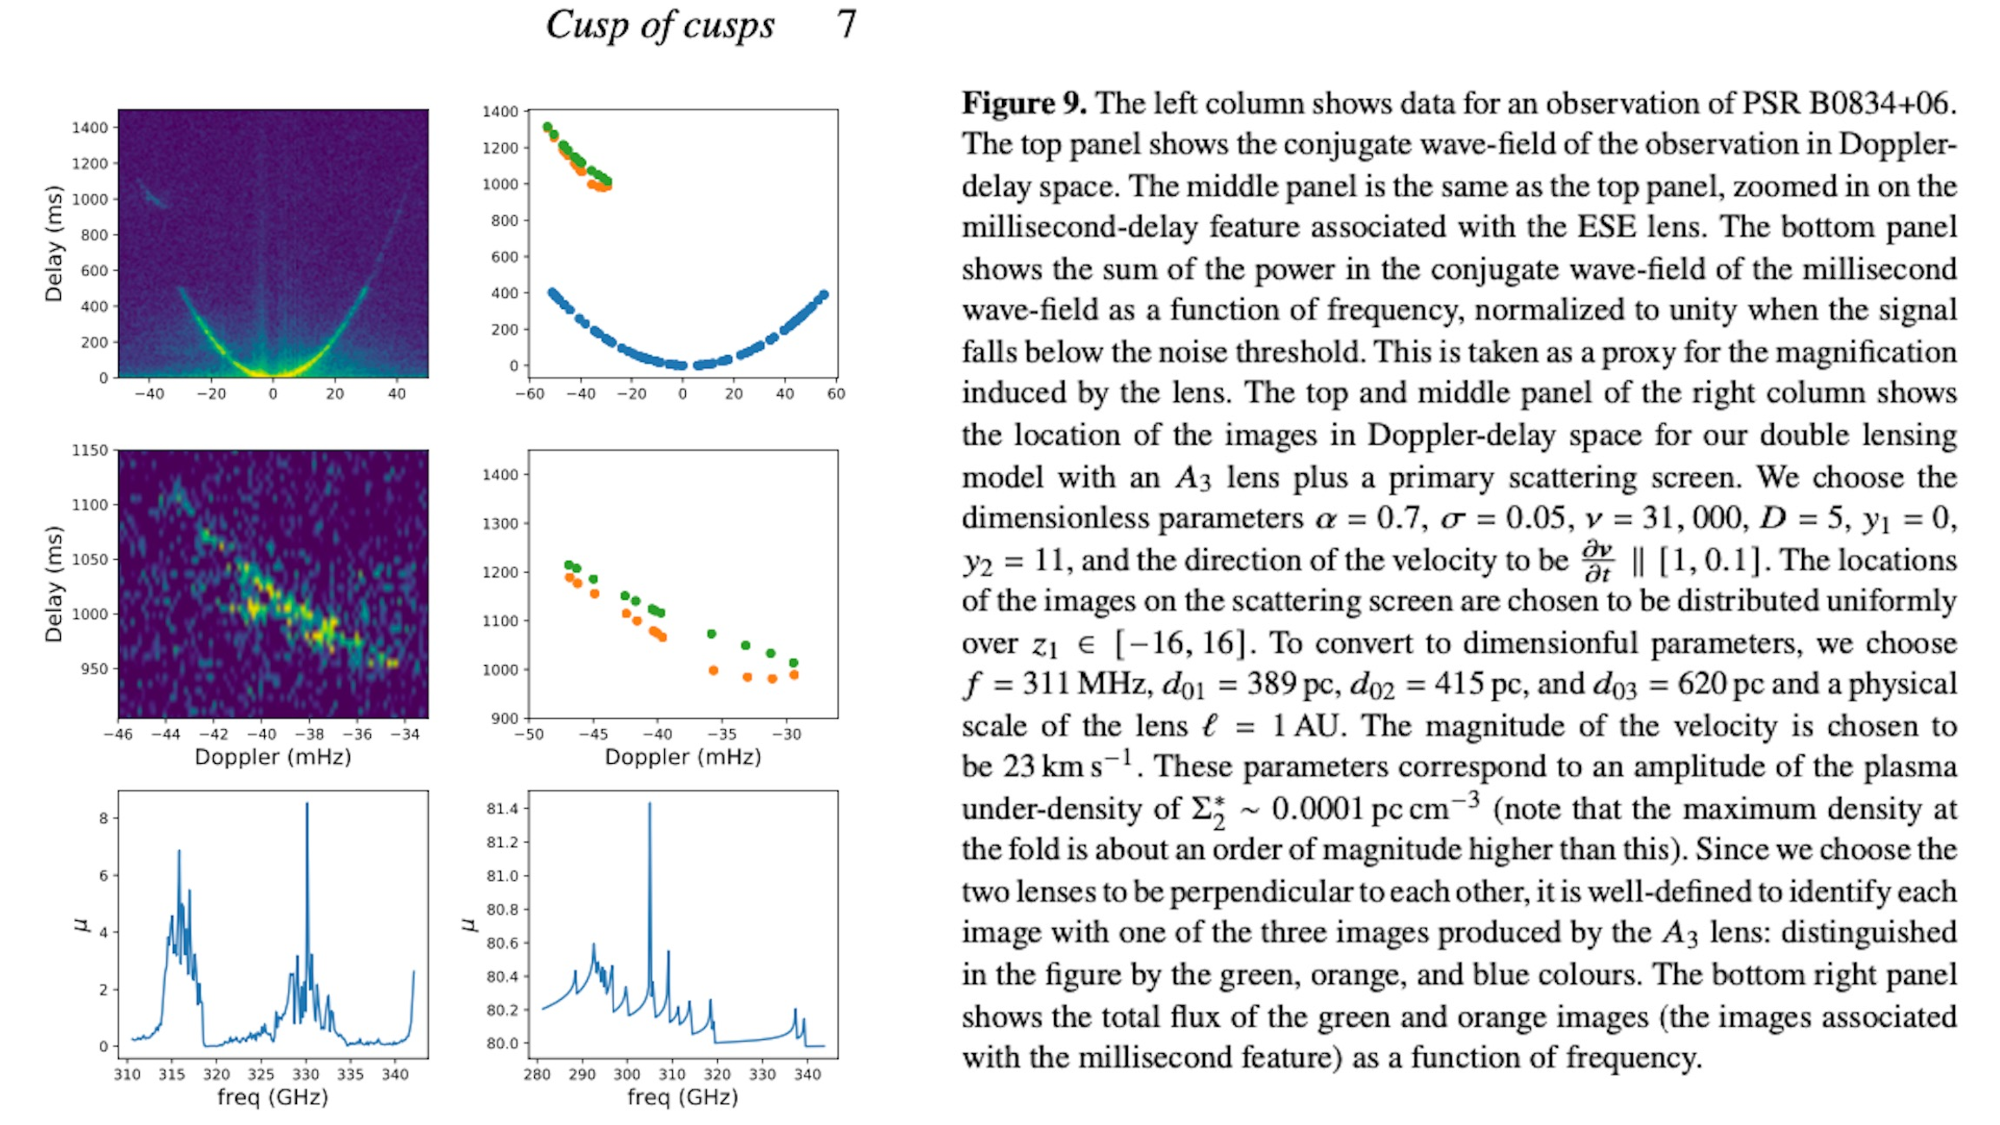
\includegraphics[width=4.65in]{Figures/esemodel.pdf}
\end{center}
  }




  \frame{
%\vspace{-0.5in}
    \frametitle{Summary}
    \begin{itemize}
     \item Many pulsars exhibit highly 1-D lensing, local in distance
     \item inverted arclets correspond to isolated lensed images
      \item ISM plasma screens modelled quantitatively as localized
        folds on sheets (c.f. Goldreich+Shridhar 2006) 
      \item questions: measuring surfaces in ISM? 
      \item potential: measure differential RM, DM in images?
      \item magnetic domain boundaries, reconnection sheets?
    \end{itemize}
  }

\end{document}
